\documentclass[11pt, oneside]{article}   	% use "amsart" instead of "article" for AMSLaTeX format
\usepackage{geometry}                		% See geometry.pdf to learn the layout options. There are lots.
\geometry{letterpaper}                   		% ... or a4paper or a5paper or ... 
%\geometry{landscape}                		% Activate for rotated page geometry
%\usepackage[parfill]{parskip}    		% Activate to begin paragraphs with an empty line rather than an indent
\usepackage{graphicx}				% Use pdf, png, jpg, or eps§ with pdflatex; use eps in DVI mode
								% TeX will automatically convert eps --> pdf in pdflatex		
\usepackage{amssymb}
\usepackage{amsmath,amssymb,amsthm,amsfonts,hyperref,fancyhdr,graphicx,subfig,bbm,multirow,array,longtable}

%SetFonts

%SetFonts

\title{Deep Learning}
\author{Bastien BRIER\\ bastien.brier@student.ecp.fr}
\date{March 5, 2017}				% Activate to display a given date or no date

\begin{document}
\maketitle
\vspace{-10pt}
\begin{center}
{\LARGE \bf Final Assignment NLP}\\
\vspace{10pt}
\end{center}

\section{Word and sentences embeddings with word2vec}
\vspace{4pt}

To begin, just a precision about the versions of gensim and keras we used.\\
\indent - gensim : 0.13.3\\
\indent - keras : 1.2.0

\subsection{Question 1}

From the info shown while training, we can see that:\\
\indent 1. There are 17,005,207 raw words in the corpus.\\
\indent 2. 16,718,844 of them are retained in the word2vec vocabulary after min\_count = 5.

\subsection{Question 2}
1. We load the two given models, and compute the similarities between different words:\\
\indent - 'apple' and 'mac' : 0.5679\\
\indent - 'apple' and 'peach' : 0.1784\\
\indent - 'banana'  and 'peach': 0.6887\\
In my opinion, we are asked about these words to show that context is really important for the algorithm to understand the word. The word 'apple' is both a fruit and the brand that has created MacBooks. And, as this word is more used as the brand name, the algorithm does not seem to acknowledge the fact that this is also a fruit, the similarity score between 'apple' and 'peach' being very low.\\
\\
2. We compute the closest word of 'difficult' with the two models:\\
\indent - model: 'easy' : 0.7629\\
\indent - model\_phrase: 'very difficult' : 0.8704\\
From these similarities, we can perceive the difference between the models. Model gives the most similar words, whereas model\_phrase computes the most similar group of words (phrases) to the word we are looking for.\\
Then, we can compute the three most similar phrases to the word 'clinton':\\
\indent - 'bush' : 0.8667\\
\indent - 'reagan' : 0.8594\\
\indent - 'gore' : 0.8575\\
\\
3. We now look for the closest word to the vector "vect(france) - vect(germany) + vect(berlin)":\\
\indent - 'paris' : 0.7577\\
\\
4. We explored a bit the embedding space and found some interesting behaviors.\\
For instance, hollywood is here much more correlated with the movie industry and the algorithm has trouble relating it as a neighborhood of Los Angeles:\\
\indent - 'hollywood' and 'batman' : 0.8004\\
\indent - 'hollywood' and 'los\_angeles' : 0.5804\\
In another subject, the vector "vect(napoleon) - vect(france) + vect(germany)" outputs:\\
\indent - 'hitler' : 0.6917\\
I also explored if relationships between music bands were known and the result is not that bad:\\
\indent - 'rolling\_stones' and 'pink\_floyd' : 0.8257\\
\indent - 'rolling\_stones' and 'beatles' : 0.8029\\
\indent - 'rolling\_stones' and 'led\_zeppelin' : 0.7991

\subsection{Question 3}

We now want to construct sentence embeddings from word embeddings, by simply taking the mean of the word embeddings. The vector is computed as :\\
	\[\begin{split}
		avgword2vec(s) = \frac{\sum_{i=1}^{S}\alpha_{i}word2vec(\omega_{i})}{\sum_{i=1}^{S}\alpha_{i}}
	\end{split}\]
\\
1. We created the function cosine\_similarity that we define as :\\
	\[\begin{split}
		cosine\_similarity(a,b) = \frac{\sum_{i=1}^{S}a_{i}b_{i}}{\sqrt{\sum_{i=1}^{S}a_{i}^{2}}\sqrt{\sum_{i=1}^{S}b_{i}^{2}}}
	\end{split}\]
With this definition, we computed the closest sentence to the sentence with idx "777" : "a girl trying to get fit for a bodybuilding competition". And the result is:\\
\indent - "gymnasts get ready for a competition" : 0.9029\\
\\
2. We filled the blanks of the most\_5\_similar function and computed then the 5 closest sentences to the same sentence as the question above :\\
\indent - "gymnasts get ready for a competition" : 0.9029\\
\indent - "a woman is getting ready to perform a song for the audience" : 0.8901\\
\indent - "a runner in a competition want to go to the finish line" : 0.8555\\
\indent - "men working to build a fence for customers" : 0.8515\\
\indent - "a man prepares to give a speech for a television audience" : 0.8495

\subsection{Question 4}

1. We now use a new technique and define the weights $\alpha_{i}$ as the IDF (Inverse Document Frequency) of each word. IDF is defined as:\\
	\[\begin{split}
		idf(t,D) = log\frac{N}{|\{d \in D : t \in d\}|}
	\end{split}\]
N is the total number of documents, and $|\{d \in D : t \in d\}|$ is the total number of documents where t appears.\\
We compute the IDF scores of different words:\\
\indent - "the" : 0.6631\\
\indent - "a" : 0.1018\\
\indent - "clinton" : this word is not in the corpus\\
\\
2. We now compute a new function taking as weights the IDF we just calculated:\\
	\[\begin{split}
		IDF\_avgword2vec(s) = \frac{\sum_{i=1}^{S}idf(\omega_{i})\cdot word2vec(\omega_{i})}{\sum_{i=1}^{S}idf(\omega_{i})}
	\end{split}\]
The closest sentence to sentence with idx 777 is now:\\
\indent - "gymnasts get ready for a competition" : 0.8961

\newpage
\section{Simple LSTM for sequence classification}
\vspace{4pt}

\subsection{Question 1}
The objective of this part is to train an LSTM for sequence classification. Here are the different shapes asked:\\
\indent 1. input of the embedding layer : 2D tensor with shape (nb\_samples, sequence\_length), here (32, 80).\\
\indent 2. input of the LSTM layer : 3D tensor with shape (nb\_samples, timesteps, input\_dim), here (32, 80, 32).\\
\indent 3. output of the LSTM layer : 2D tensor with shape (nb\_samples, output\_dim), in our case (32, 64).

\subsection{Question 2}

From the output of the lstm\_imdb.py script, we can see that there are:\\
\indent - 504,897 total parameters\\
\indent - 35,000 sentences in the training set\\
We have in this case much more parameters than number of samples. For our analysis to be possible, we have to bet on sparsity, which means that in high dimension, most of the variables will not be significant. We then have to regularize and chose variables, using techniques like lasso (L1-regularization) for instance.

\subsection{Question 3}

The exact form of $f(h_{1}, . . . ,h_{T})$ in the python script is an average pooling of the outputs of the T memory cells of the LSTM.\\
The output is computed as follows:
	\[\begin{split}
		o_{t} &= \sigma(W_{o}x_{t} + U_{o}h_{t-1} + b_{o})\\
		h_{t} &= o_{t} * tanh(C_{t})
	\end{split}\]
With $C_{t}$ being the memory cell state at time t, $x_{t}$ being $t^{th}$ input, $W_{o}$ and $U_{o}$ are weight matrices respectively associated to the current input and the previous output.\\
Source : Keras documentation.

\subsection{Question 4}

We run the model with and without dropout and computed the various training and validation accuracy by epoch.\\
	\begin{figure}[h]
		\centering
		\caption{Accuracy per epoch: without dropout (left) and with dropout (right)}
		\begin{tabular}[h]{cc}
			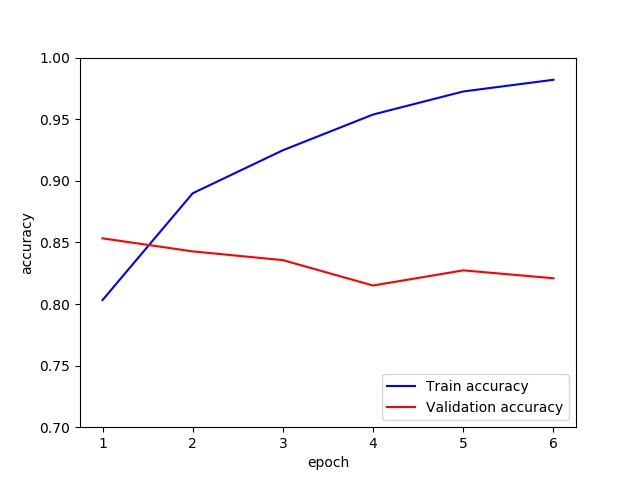
\includegraphics[width=8cm]{/Users/bastienbrier/Pictures/accuracy_w_o_dropout.jpg}
			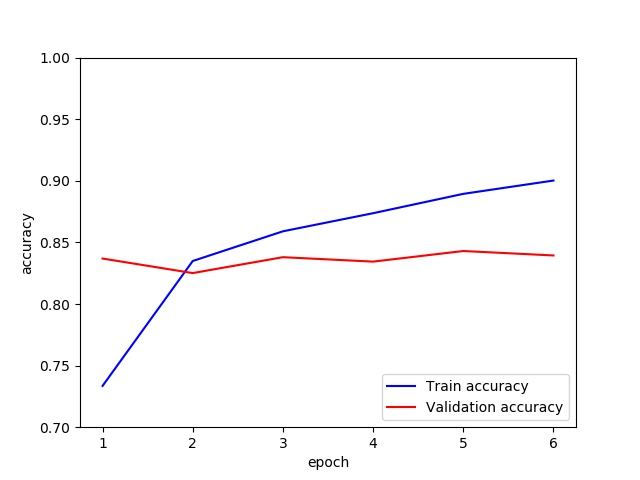
\includegraphics[width=8cm]{/Users/bastienbrier/Pictures/accuracy_w_dropout.jpg}
		\end{tabular}
	\end{figure}
\\\\
We noted also the test accuracy and loss of both models:\\
\begin{center}
\begin{tabular}{|c|c|c|}
	\hline
	  & Accuracy & Loss\\
	\hline
	Without dropout & 0.8229 & 0.6162\\
	With dropout & 0.8395 & 0.3671\\
	\hline
\end{tabular}
\end{center}
\noindent
We see that without dropout, the accuracy is much higher in the training set (goes up to 0.98), but when it comes to validation or test, the result is worst than with dropout. We can then say that dropouts prevent overfitting and give better results when it comes to validating and testing our model.

\subsection{Question 5}

Stochastic Gradient Descent (SGD) updates each parameter by subtracting the gradient of the loss multiplied by learning rate. Adaptative Moment Estimation (Adam) calculates a moving average of the first and second order moments that are also exponentially decayed. The main difference resides here, as Adam takes into account more information and keeps memory of previous states.

\newpage
\section{Simple ConvNet for sequence classification}
\vspace{4pt}

\subsection{Question 1}

We ran the script cnn\_imdb.py and here are the results obtained:\\
\indent - Test accuracy : 0.8389\\
\indent - Test score : 0.3638

\subsection{Question 2}

The difference with the previous section is that here we trained a Convolution1D. We are asked to give the shapes of the input and output:\\
\indent - input of Convolution1D : 3D tensor with shape (samples, steps, input\_dim), in this case (32, 80, 16).\\
\indent - output of Convolution1D : 3D tensor with shape (samples, new\_steps, nb\_filter), here (32, 78, 250).

\subsection{Question 3}

We created a new script, cnn\_lstm\_imdb.py, where we feed the LSTM with the output of our ConvNet (see code for more details). We then tried different combinations of parameters and here are the best results we obtained:\\
\indent - Parameters : embed\_dim = 16, nhid = 396, nb\_filter = 250, filter\_length = 3, hidden\_dims = 750, epoch = 6, dropout = 0.3\\
\indent - Test accuracy : 0.8555\\
\indent - Test score : 0.3321\\
We improved our accuracy by nearly 0.02 and score by 0.03, which is clearly not negligible, as a slight progress in the performance of the algorithm can yield much better results when used with a lot of data.

\end{document}  